\subsubsection{\stid{3.10} PEEKS} 
\paragraph{Overview} 
The PEEKS project is a focused team effort to advance the capabilities of the
ECP software stack in terms of communication-avoiding Krylov solvers and
advanced preconditioning techniques featuring fine-grained parallelism.
Previously developed techniques that are available as prototype codes -- as
well as novel algorithm developments -- are turned into production-quality 
implementations and integrated into the ECP software ecosystem 
as part of the Trilinos~\footnote{\url{https://trilinos.org/}}, the 
Ginkgo~\footnote{\url{https://github.com/ginkgo-project/ginkgo}}, and the 
MAGMA-sparse~\footnote{\url{http://icl.cs.utk.edu/magma/}} software stacks.
As leading developers of these software packages (Trilinos, Ginkgo, and 
MAGMA-sparse), the members of the PEEKS project have a strong record of 
delivering software packages that are used on future leadership-class 
supercomputers, and already now employed by ECP application projects.

In order to make the new algorithms easily accessible to ECP applications, we
in particular focus on software sustainability and cross-platform portability.
This effort is realized using sophisticated software development
and testing practices, ensuring a robust production-quality software that can
be relied upon by ECP application projects.
Delivering the production-ready preconditioner- and solver routines
via the xSDK4ECP software effort enables the ECP applications to adopt the new
technology without fundamental changes in their application design.

\paragraph{Key  Challenges}
Running iterative solvers on the next-generation HPC systems results in two 
major challenges coming from the hardware architecture:
\begin{enumerate}
\item 
Fine-grained parallelism in a single node that has to be exploited efficiently 
by the iterative solver and the preconditioner.
\item
Rising communication and synchronization cost.
\end{enumerate}

Both challenges require the redesign of existing iterative solvers with respect 
to higher parallelism within all building blocks, and a reduced number of 
communication and synchronization points. In the last few decades, numerous efforts 
have investigated the potential of communication-avoiding (CA) and pipelined 
Krylov 
solvers~\cite{yamazakiipdps2014,Cornelis2018TheCC}; however, the 
implementations 
usually 
remained in prototype status and rarely made it into production code. 
Similarly, significant effort was put into developing new preconditioning 
techniques that allow for the efficient parallelization of the preconditioner 
setup and the preconditioner 
application~\cite{chowisc2015,anzteuropa2015,ANZT20181,doi:10.1137/16M1079506}. 
Again, most implementations were 
experimental and rarely adopted by application code.

Turning the experimental code into production quality alone is rarely 
sufficient to make applications adopt the new algorithm technology, as 
application projects usually refrain from refactoring their code to integrate 
new solvers or preconditioners. This motivates a second step that is of 
comparable importance: the design of generic interfaces that allow for easy 
exchange of solver and preconditioner infrastructure without modifying the 
application code.

An important aspect for complex application codes to possess is the quick and 
comprehensive identification of performance bottlenecks. Against the background 
of integrating novel solver and preconditioning techniques, this requires 
monitoring algorithm-specific counters that provide insight about the 
appropriateness of certain parameter choices. Manual code instrumentation is 
cumbersome and practically prevents the parameter tuning in complex application 
codes. This motivates exposure of ``software-defined events'' (SDE) to external 
profiling software that is available on the target hardware.


\paragraph{Solution Strategy}

The primary thrusts of the PEEKS project are:
\begin{enumerate}
    \item \textbf{Generic numerical software interface design:}
	To propel the painless integration of new solver and preconditioner 
	technology, we design a generic interface that adheres to 
	Better Scientific Software (BSSw) design 
	principles~\cite{betterscientificsoftware}.
    The purpose of a generic interface is not restricted to the ECP effort; it is 
    anticipated to be adopted by other software efforts in the scientific 
    computing community.
	\item \textbf{Pipelined and CA Krylov methods:} 
    We realize pipelined and 
	communication-avoiding Krylov methods in production-quality code. We 
	provide interfaces and support their integration into existing application 
	codes.
	\item \textbf{Parallel preconditioning techniques:}  We implement the 
	parallel generation and application of popular preconditioning techniques 
	in production-ready code. The preconditioners are capable of leveraging the 
	parallelism available on a single node (including many-core accelerators) 
	and allow for easy integration into application codes.
    \item \textbf{Software-defined events (SDE):}  We team up with the ECP 
    Exa-PAPI project to design and realize an ecosystem for software-defined 
    events. The idea is to provide application scientists with easy access 
    to library- and solver-specific metrics via the PAPI interface. This 
    avoids cumbersome code instrumentation and library recompilation for 
    debugging algorithm behavior or identifying performance bottlenecks. 
\end{enumerate}

\paragraph{Recent Progress}
\begin{enumerate}
\item
We populated a white paper on a generic software interface in the scientific 
community and collected feedback including design modifications. The white paper 
is accessible at the PEEKS project webpage~\cite{peekswebpage}.
\item 
We deployed the production code implementation of the parallel 
generation of preconditioners based on incomplete factorization (PARILU) in the 
MAGMA-sparse software package. In an 
initial assessment of the hardware anticipated to become the backbone of the 
Summit and Sierra pre-Exascale platforms, we identified for benchmark test 
problems significant advantages over vendor-tuned functionality (see 
Figure~\ref{fig:ILUperf}).
\item
More recently, we developed a parallel threshold ILU factorization 
(ParILUT)~\cite{doi:10.1137/16M1079506}. We derived an implementation for GPU 
architectures, and deployed the production code implementation in the 
MAGMA-sparse software package.
\item 
Recently, we also realized pipeline Krylov solvers in the Trilinos 
production code ecosystem and analyzed the performance for ECP application use 
cases~\cite{1204}. A performance assessment report and slide decks documenting 
the work flow are available on the PEEKS 
webpage~\cite{peekswebpage}. 
\end{enumerate}

\begin{figure}[htb]
	\centering
	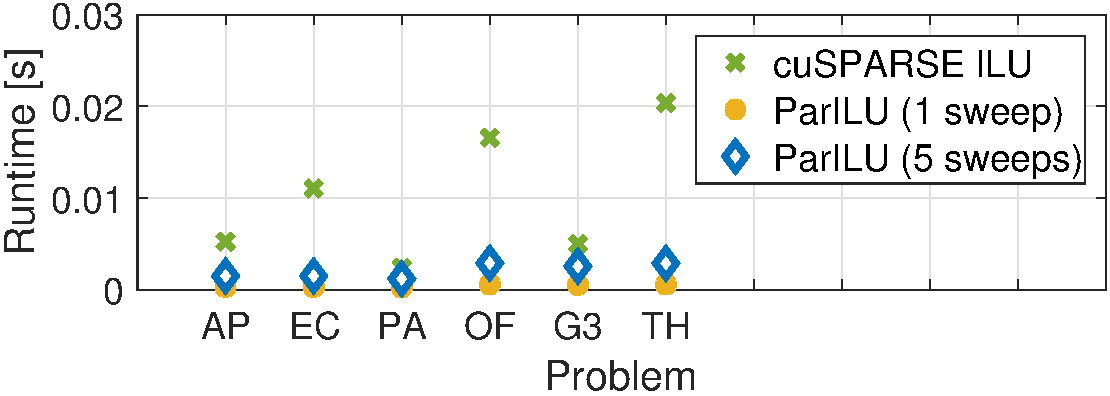
\includegraphics[width=3in]{projects/2.3.3-MathLibs/2.3.3.10-PEEKS/runtime2}
	\caption{\label{fig:ILUperf}Runtime of the ILU preconditioner generation on 
	an NVIDIA V100 GPU using the novel ParILU algorithm realized in the PEEKS 
	project and NVIDIA's cuBLAS routine, respectively.}
\end{figure}


\paragraph{Next Steps}


Our next efforts are:
\begin{enumerate}
	\item \textbf{Integrate novel algorithm functionality into ECP application 
	projects:} We are in contact with domain scientists that are willing to 
	adopt the developed pipelined Krylov solvers and parallel precondition 
	techniques to serve as production code assessment.
	\item \textbf{Integrate the software-defined events:} Together with the 
	Exa-PAPI team, we already explored the potential of software-defined events 
	(SDE) for numerical LA libraries. We next integrate these into production 
	code and assess the usability for ECP applications.
	\item \textbf{Parallel preconditioner application:} With the parallel 
	preconditioner generation being resolved, we now focus on efficient 
	preconditioner application using the parallelism available within a single 
	node. This step is strongly tied to the SDE effort, as we expect significant 
	benefits for application-tuned parameter choices in particular.
\end{enumerate}
